\documentclass{article} % 본 문서는 Article이지만 Book(책 만들때)등 가능
\usepackage[T1]{fontenc}
\usepackage{lmodern}
\usepackage{geometry}
\usepackage[hangul]{kotex} % 한글/한자 입력용
\usepackage{amsmath} % 쓰면 좋은 수식 패키지
\usepackage{amssymb} % hbar 등 제공
\usepackage{physics} % 쓰면 좋은 물리 수식 패키지
\usepackage{graphicx}
\usepackage{listings}
\usepackage{multicol}
\usepackage{forest}
\usepackage{pgf}
\usepackage{subcaption}
\graphicspath{ {./images/} }

\lstdefinestyle{mystyle}{
	numberstyle=\tiny,
	basicstyle=\ttfamily,
	showspaces=false,
	showstringspaces=false
}

\lstset{style=mystyle}

\renewcommand{\baselinestretch}{1.2} % 줄간격 1.2

\geometry{
	a4paper, % A4용지
	margin=1in % 1인치 페이지 마진
}
\usepackage[utf8]{inputenc}

\setlength\parindent{0pt}

\title {\textbf{Bayesian Approach of Fisher Discriminant Analysis} \\[1ex] \large Machine Learning Algorithms}
\author{2021024966 김희성\\2021031685 유성민}
\date{}

\begin{document}
	
\maketitle

\section{Description about FDA}
FDA(Fisher Discriminant Analysis)는 classification의 일종으로, 두 개의 class를 가장 잘 나누는 벡터 $\bf w$를 찾는 방법이다. 두 class 간의 between-class covariance는 크게, class 내부의 within-class covariance는 작게 만드는 것을 목표로 한다.

\subsection{Loss function}
두 개의 mutually exclusive class를 각각 ${\cal C}_1$, ${\cal C}_2$라 하고, 그 class의 원소의 개수를 각각 $N_1, N_2$ 이라 하자. 각 class의 mean $\boldsymbol{\mu}_1, \boldsymbol{\mu}_2$과 covariance $\Sigma_1, \Sigma_2$는 data ${\bf x}_n \in \mathbb{R}^D$에 대해 다음과 같다.

\begin{equation}
\begin{aligned}
	\boldsymbol{\mu}_1 &= \frac{1}{N_1}\sum_{n \in {\cal C}_1} {\bf x}_n \\
	\boldsymbol{\mu}_2 &= \frac{1}{N_2}\sum_{n \in {\cal C}_2} {\bf x}_n \\
	\Sigma_1 &= \frac{1}{N_1} \sum_{n \in {\cal C}_1} ({\bf x}_n - \boldsymbol{\mu}_1)({\bf x}_n - \boldsymbol{\mu}_1)^\top \\
	\Sigma_2 &= \frac{1}{N_2} \sum_{n \in {\cal C}_2} ({\bf x}_n - \boldsymbol{\mu}_2)({\bf x}_n - \boldsymbol{\mu}_2)^\top
\end{aligned}
\end{equation}

전체 data의 개수를 $N$이라 하면, $N = N_1 + N_2$ 이므로 전체 data의 mean $\boldsymbol{\mu}$는 다음과 같다.

\begin{equation}
\begin{aligned}
	\boldsymbol{\mu} &= \frac{1}{N} \sum_{n =1}^N {\bf x}_n \\
	&= \frac{1}{N} (N_1 \boldsymbol{\mu}_1 + N_2 \boldsymbol{\mu}_2)
\end{aligned}
\end{equation}

여기서 target $t_n$을 다음과 같이 정의한다.

\begin{equation}
t_n = 
\begin{cases}
	\dfrac{N}{N_1} & (n \in {\cal C}_1) \\\\
	-\dfrac{N}{N_2} & (n \in {\cal C}_2)
\end{cases}
\end{equation}

따라서 $\sum_n t_n = 0$ 이며, 이는 class label에 가중치를 두어 평균을 0으로 설정한 것으로 생각할 수 있다.\\ 

그러면, Loss function을 다음과 같이 정의할 수 있다. (Duda and Hart, 1973)

\begin{equation}
	L = \frac{1}{2} \sum_{n = 1}^N ({\bf w}^\top {\bf x}_n + w_0 - t_n)^2
\end{equation}

여기서 data ${\bf x}_n$ 을 centralize 하면 (${\bf x}_n \leftarrow {\bf x}_n - \boldsymbol{\mu}$) 새로운 mean은 $\boldsymbol{\mu} = 0$이고, bias $w_0 = - {\bf w}^\top \boldsymbol{\mu} = 0$ 이 되어 간단히 다음과 같이 쓸 수 있다.

\begin{equation}
	L = \frac{1}{2} \sum_{n = 1}^N ({\bf w}^\top {\bf x}_n - t_n)^2
	\label{eq:loss}
\end{equation}

\section{Bayesian Approach}
\subsection{Likelihood}

일반성을 잃지 않고, 모든 data는 centralized 되어 있다고 가정한다. 그러면 식 (\ref{eq:loss}) 를 사용하여 다음과 같은 likelihood를 구성할 수 있다. 

\begin{equation}
\begin{aligned}
	p(t | {\bf x}, {\bf w}) &= {\cal N} (t | {\bf w}^\top {\bf x}, \sigma^2) \\
	&= \frac{1}{\sqrt{2 \pi \sigma^2}} \exp \left(-\frac{1}{2 \sigma^2} ({\bf w}^\top {\bf x} - t)^2 \right)
\end{aligned}
\end{equation}

\subsection{Prior}

parameter ${\bf w}$에 대한 prior은 다음과 같다.

\begin{equation}
\begin{aligned}
	p({\bf w}) &= {\cal N} ({\bf w} | {\bf 0}, \sigma_{\bf w}^2 {\bf I})
\end{aligned}
\end{equation}

\subsection{Posterior}

posterior $p({\bf w} | {\cal D})$ 는 Bayes' rule에 의해 다음과 같이 구할 수 있다.

\begin{equation}
\begin{aligned}
	p({\bf w} | {\cal D}) &= p({\bf w}) p({\cal D} | {\bf w}) \\
	&= \prod_{n = 1}^N p({\bf w}) p(t_n | {\bf x}_n, {\bf w}) \\
	&= C ~ \exp( \textcircled{\scriptsize 1} )
\end{aligned}
\end{equation}

likelihood와 prior 모두 gaussian 이므로, posterior 또한 gaussian 이다. 따라서, exp 내부 항만 전개하면 다음과 같다.

\begin{equation}
\begin{aligned}
	\textcircled{\scriptsize 1} &= -\frac{1}{2\sigma^2}  \left( \sum_{n = 1}^N \left(  {\bf w}^\top{\bf x}_n{\bf x}_n^\top{\bf w} - 2 t_n {\bf w}^\top {\bf x}_n + t_n^2 \right) + \frac{\sigma^2}{\sigma_{\bf w} ^2} {\bf w}^\top {\bf w}  \right)
	\\
	&= -\frac{1}{2\sigma^2}  \left( \sum_{n \in {\cal C}_1} \left(  {\bf w}^\top{\bf x}_n{\bf x}_n^\top{\bf w} - 2 \frac{N}{N_1} {\bf w}^\top {\bf x}_n + \frac{N^2}{N_1^2} \right) + \sum_{n \in {\cal C}_2} \left(  {\bf w}^\top{\bf x}_n{\bf x}_n^\top{\bf w} + 2 \frac{N}{N_2} {\bf w}^\top {\bf x}_n + \frac{N^2}{N_2^2} \right) + \frac{\sigma^2}{\sigma_{\bf w} ^2} {\bf w}^\top {\bf w}  \right)
	\\
	&= -\frac{1}{2\sigma^2} \left(
		{\bf w}^\top \left(
			\sum_{n \in {\cal C}_1}{\bf x}_n {\bf x}_n^\top + \sum_{n \in {\cal C}_2}{\bf x}_n {\bf x}_n^\top + \frac{\sigma^2}{\sigma_{\bf w}^2} {\bf I}
		\right) {\bf w} - 2N{\bf w}^\top(\boldsymbol{\mu}_1 - \boldsymbol{\mu}_2)
	 \right) + C
\end{aligned} 
\end{equation}

여기서 \textit{within-class} covariance ${\bf S}_{\rm W}$와 \textit{between-class} covariance ${\bf S}_{\rm B}$ 를 다음과 같이 정의하자.

\begin{equation}
\begin{aligned}
	{\bf S}_{\rm W} &= \sum_{n \in {\cal C}_1} ({\bf x}_n - \boldsymbol{\mu}_1) ({\bf x}_n - \boldsymbol{\mu}_1)^\top +  \sum_{n \in {\cal C}_2} ({\bf x}_n - \boldsymbol{\mu}_2) ({\bf x}_n - \boldsymbol{\mu}_2)^\top \\
	{\bf S}_{\rm B} &= (\boldsymbol{\mu}_1 - \boldsymbol{\mu}_2)(\boldsymbol{\mu}_1 - \boldsymbol{\mu}_2)^\top
\end{aligned}
\end{equation}

그러면, 다음이 성립한다.

\begin{equation}
\begin{aligned}
	\sum_{n = 1}^N {\bf x}_n {\bf x}_n ^\top &= \sum_{n \in {\cal C}_1} {\bf x}_n {\bf x}_n^\top + \sum_{n \in {\cal C}_2} {\bf x}_n {\bf x}_n^\top \\
	&= {\bf S}_{\rm W} + N_1 \boldsymbol{\mu}_1 \boldsymbol{\mu}_1^\top + N_2 \boldsymbol{\mu}_2 \boldsymbol{\mu}_2^\top \\
	&= {\bf S}_{\rm W} + \frac{N_1 N_2}{N} {\bf S}_{\rm B} 
\end{aligned}
\end{equation}

따라서, \textcircled{\scriptsize 1} 은 다음과 같다.

\begin{equation}
\begin{aligned}
	\textcircled{\scriptsize 1} &= -\frac{1}{2\sigma^2} \left(
		{\bf w}^\top \left( {\bf S}_{\rm W} + \frac{N_1 N_2}{N} {\bf S}_{\rm B} + \frac{\sigma^2}{\sigma_{\bf w}^2}{\bf I} \right)
		{\bf w} - 2N{\bf w}^\top (\boldsymbol{\mu}_1 - \boldsymbol{\mu}_2)
	\right)  + C 
	\\\\
	&= -\frac{1}{2} ({\bf w} - \boldsymbol{\mu}_{{\bf w}|{\cal D}})^\top \Sigma_{{\bf w}|{\cal D}}^{-1} ({\bf w} - \boldsymbol{\mu}_{{\bf w}|{\cal D}}) + C
\end{aligned}
\end{equation}

즉, posterior $p({\bf w} | {\cal D})$ 는 다음과 같다.

\begin{equation}
	p({\bf w} | {\cal D}) = {\cal N} (\boldsymbol{\mu}_{{\bf w}|{\cal D}}, \Sigma_{{\bf w}|{\cal D}})
\end{equation}

여기서 $\boldsymbol{\mu}_{{\bf w} | {\cal D}}$와 $\Sigma_{{\bf w} | {\cal D}}$는 다음과 같다.

\begin{equation}
\begin{aligned}
	\boldsymbol{\mu}_{{\bf w} | {\cal D}} &= N \left( {\bf S}_{\rm W} + \frac{N_1 N_2}{N} {\bf S}_{\rm B} + \frac{\sigma^2}{\sigma_{\bf w}^2}{\bf I} \right)^{-1} (\boldsymbol{\mu}_1 - \boldsymbol{\mu}_2)
	\\
	\Sigma_{{\bf w} | {\cal D}} &= \sigma^2 \left( {\bf S}_{\rm W} + \frac{N_1 N_2}{N} {\bf S}_{\rm B} + \frac{\sigma^2}{\sigma_{\bf w}^2}{\bf I} \right)^{-1}
\end{aligned}
\end{equation}

\subsection{Predictive Distribution}
새로운 input data ${\bf x}$에 대하여 predictive distribution $p(t | {\bf x}, {\cal D})$ 는 likelihood와 posterior의 곱을 적분하여 구할 수 있다.

\begin{equation}
	p(t | {\bf x}, {\cal D}) = \int _{\cal W} p(t | {\bf x}, {\bf w}) p({\bf w} | {\cal D}) \dd{{\bf w}}
\end{equation}

이 또한 gaussian이므로, exp 내부 항만 보도록 하자. 또한, ${\bf w}$에 대해 적분한 후의 결과는 $t$에 대한 probability distribution 이므로, $p(t | {\bf x}, {\bf w}) p({\bf w} | {\cal D})$의 exp 내의 항을 다음과 같이 정리할 수 있다.

\begin{equation}
\begin{aligned}
	&-\frac{1}{2 \sigma^2} \left(
		{\bf w}^\top \left( {\bf S}_{\rm W} + \frac{N_1 N_2}{N} {\bf S}_{\rm B} + \frac{\sigma^2}{\sigma_{\bf w}^2}{\bf I} \right)
		{\bf w} - 2N{\bf w}^\top (\boldsymbol{\mu}_1 - \boldsymbol{\mu}_2) + ({\bf w}^\top {\bf x} - t)^2
	 \right) + \cdots 
	 \\
	 =& -\frac{1}{2 \sigma^2} \left(
	 {\bf w}^\top \underbrace{\left( {\bf x}{\bf x}^\top +  {\bf S}_{\rm W} + \frac{N_1 N_2}{N} {\bf S}_{\rm B} + \frac{\sigma^2}{\sigma_{\bf w}^2}{\bf I} \right)}_{\Delta}
	 {\bf w} - 2N{\bf w}^\top (\boldsymbol{\mu}_1 - \boldsymbol{\mu}_2 + t{\bf x}/N) + t^2
	 \right) + \cdots 
\end{aligned}
\end{equation}

여기서 ${\bf w}$를 marginalize out 시키면 $t$에 대한 gaussian distribution 을 얻을 수 있고, 그것의 exp 내부 항은 다음과 같다.

\begin{equation}
\begin{aligned}
	&-\frac{1}{2 \sigma^2} \left(
		(1 - {\bf x}^\top \Delta^{-1} {\bf x})t^2 - 2N {\bf x}^\top \Delta ^{-1} (\boldsymbol{\mu}_1 - \boldsymbol{\mu}_2)t
	\right) + \cdots
	\\\\
	=& \frac{(1 - {\bf x}^\top \Delta^{-1} {\bf x})}{2\sigma^2} \left(
		t - \frac{N{\bf x}^\top \Delta^{-1} (\boldsymbol{\mu}_1 - \boldsymbol{\mu}_2)}{(1 - {\bf x}^\top \Delta^{-1} {\bf x})}
	\right)^2
\end{aligned}
\end{equation}

따라서, prediction의 mean과 variance는 다음과 같다.

\begin{equation}
\begin{aligned}
	\mathbb{E}[t | {\bf x}, {\cal D}] &= \cfrac{N {\bf x}^\top \left( {\bf x}{\bf x}^\top + {\bf S}_{\rm W} + \dfrac{N_1 N_2}{N} {\bf S}_{\rm B} + \dfrac{\sigma^2}{\sigma^2_{\bf w}} {\bf I}\right)^{-1}(\boldsymbol{\mu}_1 - \boldsymbol{\mu}_2)}{1 - {\bf x}^\top \left( {\bf x}{\bf x}^\top + {\bf S}_{\rm W} + \dfrac{N_1 N_2}{N} {\bf S}_{\rm B} + \dfrac{\sigma^2}{\sigma^2_{\bf w}} {\bf I}  \right)^{-1} {\bf x}}
	\\\\
	{\rm Var}[t | {\bf x}, {\cal D}] &= \cfrac{\sigma^2}{1 - {\bf x}^\top \left( {\bf x}{\bf x}^\top + {\bf S}_{\rm W} + \dfrac{N_1 N_2}{N} {\bf S}_{\rm B} + \dfrac{\sigma^2}{\sigma^2_{\bf w}} {\bf I}  \right)^{-1} {\bf x}}
\end{aligned}
\label{eq:evar}
\end{equation}

여기서 다음과 같은 행렬 ${\bf X}$를 도입하자.

\begin{equation}
	{\bf X} = \begin{pmatrix}
		\vrule & & \vrule \\
		{\bf x}_1 & \cdots & {\bf x}_N \\
		\vrule & & \vrule
	\end{pmatrix} \in \mathbb{R}^{D \times N}
\end{equation}

그러면 다음이 성립한다.

\begin{equation}
\begin{aligned}
	\sum_{n=1}^N {\bf x}_n {\bf x}_n^\top &= {\bf S}_{\rm W} + \frac{N_1 N_2}{N} {\bf S}_{\rm B}  \\
	&= {\bf X}{\bf X}^\top
\end{aligned}
\end{equation}

따라서, 식 (\ref{eq:evar}) 은 다음과 같이 간단히 쓸 수 있다.

\begin{equation}
\begin{aligned}
	\mathbb{E}[t | {\bf x}, {\cal D}] &= \cfrac{N {\bf x}^\top \left( {\bf x}{\bf x}^\top + {\bf X}{\bf X}^\top + \dfrac{\sigma^2}{\sigma^2_{\bf w}} {\bf I}\right)^{-1}(\boldsymbol{\mu}_1 - \boldsymbol{\mu}_2)}{1 - {\bf x}^\top \left( {\bf x}{\bf x}^\top + {\bf X}{\bf X}^\top + \dfrac{\sigma^2}{\sigma^2_{\bf w}} {\bf I}  \right)^{-1} {\bf x}}
	\\\\
	{\rm Var}[t | {\bf x}, {\cal D}] &= \cfrac{\sigma^2}{1 - {\bf x}^\top \left( {\bf x}{\bf x}^\top + {\bf X}{\bf X}^\top + \dfrac{\sigma^2}{\sigma^2_{\bf w}} {\bf I}  \right)^{-1} {\bf x}}
\end{aligned}
\label{eq:evar1}
\end{equation}

식 (\ref{eq:evar1}) 의 분모를 비교해보면 같다는 것을 알 수 있다. 이를 Woodbury identity를 이용하여 정리하면 다음과 같다.


\begin{align}
	({\rm denom}) &= \left(
		1 + {\bf x}^\top \left( 
			{\bf X}{\bf X}^\top + \frac{\sigma^2}{\sigma^2_{\bf w}} {\bf I}
		\right) ^{-1} {\bf x}
	\right) ^{-1} \label{eq:den1} \\
	&= \left(
		1 + \frac{\sigma^2_{\bf w}}{\sigma^2} \left(
			{\bf x}^\top {\bf x} - {\bf x}^\top {\bf X} \left( 
				{\bf X}^\top{\bf X} + \frac{\sigma^2}{\sigma^2_{\bf w}}
			\right) {\bf X}^\top {\bf x}
		\right)
	\right) \label{eq:den2}
\end{align}


식 (\ref{eq:den2}) 를 variance에 plugin 하면 다음과 같다.

\begin{equation}
\begin{aligned}
	{\rm Var}[t | {\bf x}, {\cal D}] &= \sigma^2 + \sigma^2_{\bf w} {\bf x}^\top{\bf x} - \sigma^2_{\bf w} {\bf x}^\top {\bf X} \left( {\bf X}^\top{\bf X} + \frac{\sigma^2}{\sigma^2_{\bf w}} {\bf I} \right)^{-1} {\bf X}^\top {\bf x} \\
	&\ge \sigma^2
\end{aligned}
\end{equation}

mean 의 분자에 Woodbury identity를 적용하면 다음과 같다.

\begin{equation}
\begin{aligned}
	({\rm num}) = N{\bf x}^\top \left(
		{\bf X}{\bf X}^\top + \dfrac{\sigma^2}{\sigma^2_{\bf w}} {\bf I}
	\right)^{-1} (\boldsymbol{\mu}_1 - \boldsymbol{\mu}_2) -
	\cfrac{N{\bf x} ^\top \left({\bf X}{\bf X}^\top + \dfrac{\sigma^2}{\sigma^2_{\bf w}} {\bf I} \right)^{-1} {\bf x}{\bf x}^\top \left({\bf X}{\bf X}^\top + \dfrac{\sigma^2}{\sigma^2_{\bf w}} {\bf I} \right)^{-1} (\boldsymbol{\mu}_1 - \boldsymbol{\mu}_2)}{1 + {\bf x}^\top \left({\bf X}{\bf X}^\top + \dfrac{\sigma^2}{\sigma^2_{\bf w}} {\bf I} \right)^{-1}{\bf x}}
\end{aligned}
\end{equation}

분모에 식 (\ref{eq:den1}) 을 plugin 하여 정리하면 mean은 다음과 같다.

\begin{equation}
	\mathbb{E}[t | {\bf x}, {\cal D}] = N{\bf x}^\top \left(
	{\bf X}{\bf X}^\top + \dfrac{\sigma^2}{\sigma^2_{\bf w}} {\bf I}
	\right)^{-1} (\boldsymbol{\mu}_1 - \boldsymbol{\mu}_2)
	\label{eq:mean}
\end{equation}

\subsection{Result}

\begin{figure}[ht]
\begin{subfigure}{.5\textwidth}
	\centering
	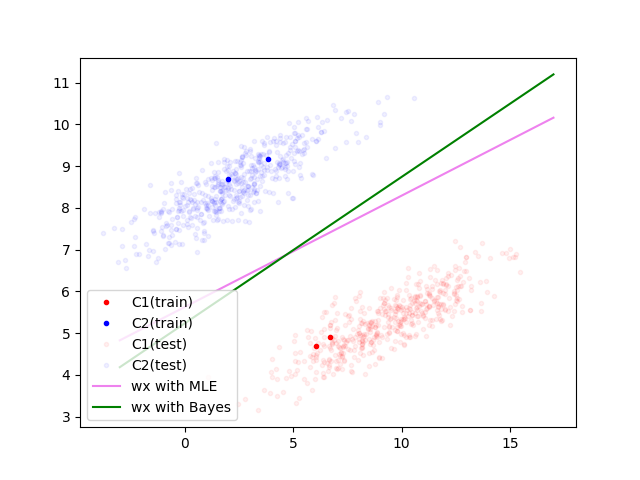
\includegraphics[width=\textwidth]{Figure_4.png}
	\caption{Well classified}
	\label{fg:fda1}
\end{subfigure}
\begin{subfigure}{.5\textwidth}
	\centering
	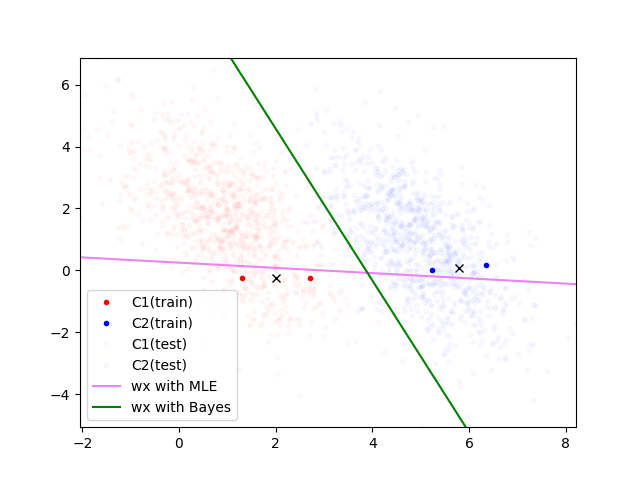
\includegraphics[width=\textwidth]{Figure_7.png}
	\caption{Good with Bayesian, Bad for MLE}
	\label{fg:fda2}
\end{subfigure}
\begin{subfigure}{.5\textwidth}
	\centering
	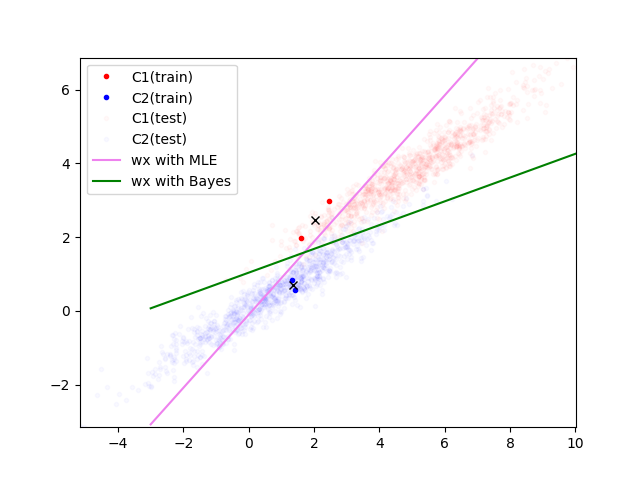
\includegraphics[width=\textwidth]{Figure_5.png}
	\caption{Good with Bayesian, Bad for MLE}
	\label{fg:fda3}
\end{subfigure}
\begin{subfigure}{.5\textwidth}
	\centering
	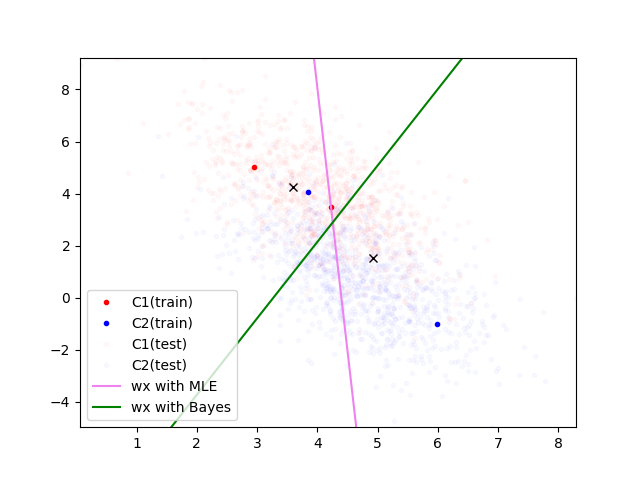
\includegraphics[width=\textwidth]{Figure_6.png}
	\caption{Slightly outlying training data}
	\label{fg:fda4}
\end{subfigure}
\caption{Result of FDA with MLE \& Bayesian ($\sigma^2 / \sigma^2_{\bf w} = 0.1$)}
\label{fg:fdares}
\end{figure}

그림 \ref{fg:fdares} 은 MLE를 이용해 구한 $\bf w$와 Bayesian approach를 이용해 구한 $\bf w$를 비교한 결과이다. 진한 점은 training data이고, 연한 점은 test data이다. 또한, 분홍색 실선은 MLE로 구한 boundary 이고 녹색 실선은 Bayesian approach로 구한 boundary 이다.\\ 

극단적인 성능 비교를 위하여, training data의 개수를 각 class 당 2개\footnote{1개로 하면 MLE에서 singular matrix가 생기기 때문에 불가능하다.}로 설정하였다. 그림 \ref{fg:fda1} 과 같이 MLE와 Bayesian classifier가 모두 잘 분류하는 경우도 있는 반면, 대부분의 상황에서 그림 \ref{fg:fda2}, \ref{fg:fda3} 과 같이 Bayesian boundary가 더 잘 분류함을 확인할 수 있다. 자세히는, MLE로 생성된 boundary는 over-fitted 된 것을 확인할 수 있는 반면, Bayesian으로 생성된 boundary는 비교적 덜 그렇다는 것을 확인할 수 있다. 이는 Bayesian approach 에서 사용된 prior variance 가 regularization term 역할을 했기 때문으로 사료된다. \\ 

또한, 그림 \ref{fg:fda4} 와 같이 training data가 약간 outlying 하여도 MLE에 비해 Bayesian이 더 좋은 classification을 하는 것을 확인할 수 있었다.

\section{Kernel Extension}

다음과 같은 mapping function $\phi$ 에 대해:
\begin{equation}
	\phi: \mathbb{R}^D \to \mathbb{R}^M
\end{equation}

mapping 된 data $\phi({\bf x}) \in \mathbb{R}^M$를 생각하자. 그러면, 이렇게 mapping 된 data의 mean을 다음과 같이 정의한다.

\begin{equation}
\begin{aligned}
	\boldsymbol{\mu}_1^\phi &= \frac{1}{N_1} \sum_{n \in {\cal C}_1} \phi({\bf x}_n) \\
	\boldsymbol{\mu}_2^\phi &= \frac{1}{N_2} \sum_{n \in {\cal C}_2} \phi({\bf x}_n)
\end{aligned}
\end{equation}

여기서 mapped data를 centralized 해주면, loss function은 다음과 같다.

\begin{equation}
	\frac{1}{2} \sum_{n = 1}^N ({\bf w}^\top \phi({\bf x}_n) - t_n)^2
\end{equation} 

다음과 같은 행렬을 도입하자.
\begin{equation}
\begin{aligned}
	\boldsymbol{\Phi} &= \begin{pmatrix}
		\vrule & & \vrule \\
		\phi({\bf x}_1) & \cdots & \phi({\bf x}_N) \\
		\vrule & & \vrule
	\end{pmatrix} \in \mathbb{R}^{M \times N} \\\\
	{\bf t} &= (t_1, \cdots, t_N)^\top \in \mathbb{R}^{N}
\end{aligned}
\end{equation}

또한, positive definite function $k$에 대하여, 다음 행렬을 정의하자.
\begin{equation}
\begin{aligned}
	k({\bf x}_i, {\bf x}_j) &= \phi({\bf x}_i)^\top \phi({\bf x}_j)
	\\\\
	{\bf K} &= \begin{pmatrix}
		k({\bf x}_1, {\bf x}_1) & \cdots & k({\bf x}_1, {\bf x}_N) \\
		\vdots & \ddots & \vdots \\
		k({\bf x}_N, {\bf x}_1) & \cdots & k({\bf x}_N, {\bf x}_N)
	\end{pmatrix} \\\\
	{\bf k} &= (k({\bf x}, {\bf x}_1), \cdots, k({\bf x}, {\bf x}_N))^\top 
\end{aligned}
\end{equation}

여기서, 식 (\ref{eq:mean}) 은 다음과 같이 변형할 수 있으므로:
\begin{equation}
	\mathbb{E}[t | {\bf x}, {\cal D}] = {\bf x}^\top {\bf X} \left(
	{\bf X}^\top{\bf X} + \dfrac{\sigma^2}{\sigma^2_{\bf w}} {\bf I}
	\right)^{-1} {\bf t}
	\label{eq:mean2}
\end{equation}

mapping 된 data의 predictive distribution의 mean과 variance는 각각 다음과 같다.

\begin{equation}
\begin{aligned}
	\mathbb{E}[t | {\bf x}, {\cal D}] &= \phi({\bf x})^\top\boldsymbol{\Phi} \left(
	\boldsymbol{\Phi}^\top \boldsymbol{\Phi} + \dfrac{\sigma^2}{\sigma^2_{\bf w}} {\bf I}
	\right)^{-1} {\bf t}
	\\
	&=  {\bf k}^\top \left( {\bf K} + \frac{\sigma^2}{\sigma^2_{\bf w} } {\bf I} \right)^{-1} {\bf t} \\
	{\rm Var}[t | {\bf x}, {\cal D}] &= \sigma^2 + \sigma^2_{\bf w} \phi({\bf x})^\top\phi({\bf x}) - \sigma^2_{\bf w} \phi({\bf x})^\top \boldsymbol{\Phi} \left( \boldsymbol{\Phi}^\top\boldsymbol{\Phi} + \frac{\sigma^2}{\sigma^2_{\bf w}} {\bf I} \right)^{-1} \boldsymbol{\Phi}^\top \phi({\bf x}) \\
	&= \sigma^2 + \sigma^2_{\bf w} k({\bf x}, {\bf x}) - \sigma^2_{\bf w} {\bf k}^\top \left( {\bf K} + \frac{\sigma^2}{\sigma^2_{\bf w}} {\bf I} \right)^{-1} {\bf k}
\end{aligned}
\end{equation}

이는 kernel vector ${\bf k}'$과 kernel matrix ${\bf K}'$ 이 다음과 같은 \textbf{Gaussian process} 라고 생각할 수 있다.

\begin{equation}
\begin{aligned}
	{\bf k}'_{i} &= \sigma^2_{{\bf w}} \phi({\bf x})^\top \phi({\bf x}_i) \\
	{\bf K}'_{ij} &= \sigma^2_{\bf w} \phi({\bf x}_i)^\top \phi({\bf x}_j) + \sigma^2 \delta_{ij}
\end{aligned}
\end{equation}

\subsection{Result}

\begin{figure}[ht]
	\begin{subfigure}{.5\textwidth}
		\centering
		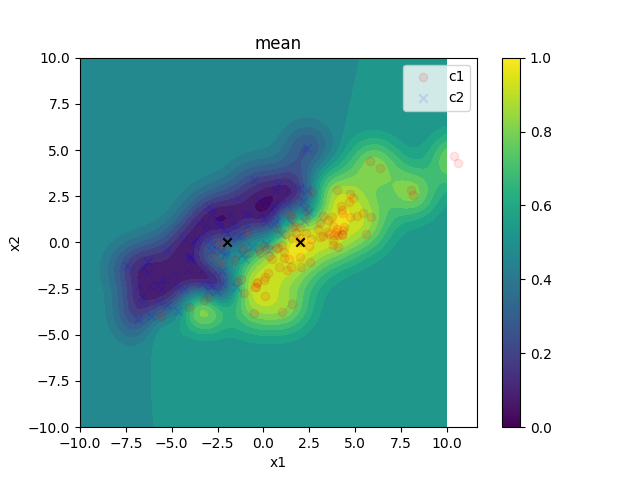
\includegraphics[width=\textwidth]{Kernel_1.png}
		\caption{Mean of classifier}
		\label{fg:ker1}
	\end{subfigure}
	\begin{subfigure}{.5\textwidth}
		\centering
		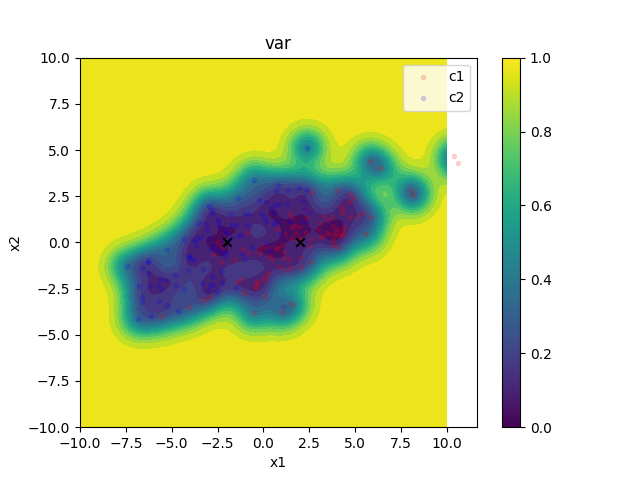
\includegraphics[width=\textwidth]{Kernel_2.png}
		\caption{Variance of classifier}
		\label{fg:ker2}
	\end{subfigure}
	\caption{Result of Kernel-extended Bayesian FDA}
	\label{fg:kernels}
\end{figure}

그림 \ref{fg:kernels} 는 kernel-extended Bayesian FDA의 결과를 나타낸 것으로, Gaussian process를 이용한 classification으로 볼 수 있다. Kernel function으로는 Gaussian kernel에 Bayesian approach로 얻어진 regularization term 을 추가한 것을 사용하였다. \\

그림 \ref{fg:ker1} 를 보면 각 class의 data가 잘 분류되었음을 확인할 수 있다. 단순히 하나의 linear boundary를 제공하는 FDA에 비해 훨씬 정교하게 분류됨을 확인할 수 있다. 또한, regularization term이 자연스럽게 추가되어서 이상치나 적은 data에 강한 것을 확인할 수 있다. \\

그림 \ref{fg:ker2} 는 classifier의 variance를 나타낸 것으로, data가 있는 곳의 variance는 작고, 그것으로부터 멀어질 수록 증가하는 gaussian process 의 특징을 확인할 수 있다. 또한, regularization term 덕분에 극단적으로 variance가 낮은 점이 없다는 것도 확인할 수 있다.

\section{References}
Bishop, C. M. (2006). \textit{Pattern Recognition and Machine Learning}. New York :Springer.

Duda, R. O. and P. E. Hart (1973). Pattern Classification and Scene Analysis. Wiley.




















\end{document}

